\documentclass[journal]{IEEEtran}
\usepackage[english]{babel}

\usepackage{amssymb, amsmath} %Paquetes matemáticos de la American Mathematical 
\usepackage[utf8]{inputenc}
\usepackage{graphicx}
\usepackage{float}
\usepackage{hyperref}
\usepackage{listings}
\usepackage{xcolor}

\definecolor{codegreen}{rgb}{0,0.6,0}
\definecolor{codegray}{rgb}{0.5,0.5,0.5}
\definecolor{codepurple}{rgb}{0.58,0,0.82}
\definecolor{backcolour}{rgb}{0.95,0.95,0.92}
% Definicio de estilo para el codigo fuente que se cita
\lstdefinestyle{mystyle}{
    backgroundcolor=\color{backcolour},   
    commentstyle=\color{codegreen},
    keywordstyle=\color{magenta},
    numberstyle=\tiny\color{codegray},
    stringstyle=\color{codepurple},
    basicstyle=\ttfamily\footnotesize,
    breakatwhitespace=false,         
    breaklines=true,                 
    captionpos=b,                    
    keepspaces=true,
    numbers=left,                    
    numbersep=5pt,                  
    showspaces=false,                
    showstringspaces=false,
    showtabs=false,                  
    tabsize=2,
}
\lstset{style=mystyle}

\renewcommand{\lstlistingname}{Código}

\ifCLASSINFOpdf

\else

\fi
\begin{document}

\title{Ejercicio 4 - tema 6 \\ Explorar tablespaces}
%
\author{Vicente Romero Andrade}

\markboth{Ejercicio 4 - tema 6 Explorar tablespaces, Julio~2021}%
{Shell \MakeLowercase{\textit{et al.}}: }
% The only time the second header will appear is for the odd numbered pages

\maketitle


\IEEEpeerreviewmaketitle

\section{Objetivo}
% The very first letter is a 2 line initial drop letter followed

\IEEEPARstart{E}{l} objetivo es familiarizarse con el concepto de tablespace. 
Explorar las principales vistas del diccionario de datos que muestran información asociada con los
tablespaces existentes en una base de datos así como los tablespaces a los que un usuario tiene acceso: default, temporal e undo.

\section{Desarrollo}
\subsection{sentencias}
\begin{lstlisting}[language=sql, caption=s-00-consulta-tablespaces.sql,label={lst:codigo1}]
  whenever sqlerror exit rollback
  set serveroutput on
  connect sys/system2 as sysdba
  --A
  select
    TABLESPACE_NAME,
    BLOCK_SIZE,
    INITIAL_EXTENT,
    NEXT_EXTENT,
    MAX_SIZE,
    STATUS,
    CONTENTS,
    LOGGING
  from DBA_TABLESPACES
  --B
  select
    TABLESPACE_NAME,
    EXTENT_MANAGEMENT,
    SEGMENT_SPACE_MANAGEMENT,
    BIGFILE,
    ENCRYPTED
  from DBA_TABLESPACES;
  --C
  select
         D.USERNAME,
         D.DEFAULT_TABLESPACE,
         D.TEMPORARY_TABLESPACE,
         trunc(DT.BYTES/(1024*1024),2) as QUOTA_MB,
         DT.BLOCKS
  from DBA_USERS D
      join DBA_TS_QUOTAS DT
          on DT.USERNAME = D.USERNAME;
  whenever sqlerror continue
  
\end{lstlisting}
\begin{figure}[H]
  \centering
  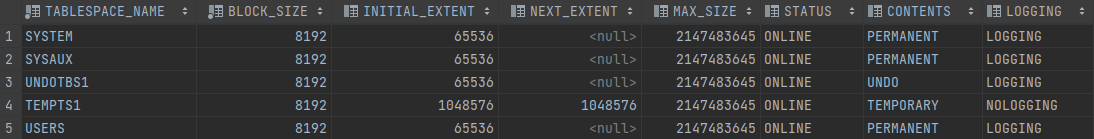
\includegraphics[scale=.22]{captura_1.png}
   \caption{Salida punto A}
   \label{fig:validador_1}
\end{figure}
\begin{figure}[H]
  \centering
  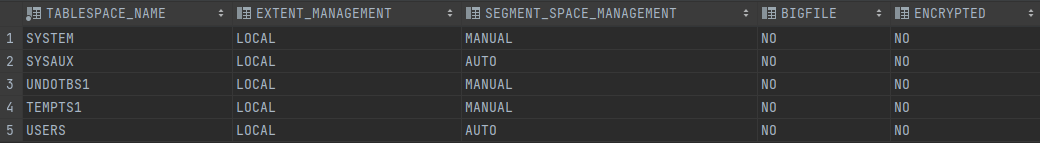
\includegraphics[scale=.22]{captura_2.png}
   \caption{Salida punto B}
   \label{fig:validador_2}
\end{figure}
\begin{figure}[H]
  \centering
  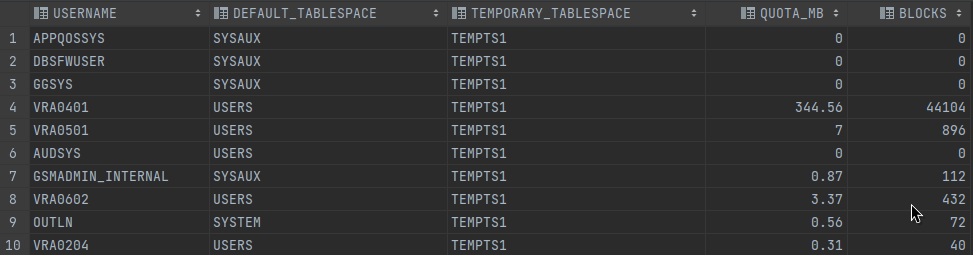
\includegraphics[scale=.22]{captura_3.png}
   \caption{Salida punto C}
   \label{fig:validador_3}
\end{figure}

\section{Conclusiones}
Se comprendio de manera exitosa el concepto de tablespaces, para esto se exploraron las vistas y 
tablas del diccionario de datos asociadas a las mismas.
\ifCLASSOPTIONcaptionsoff
  \newpage

\fi

\end{document}
